
% cristalli in PET, Quenching, optical ( Rayleigh)

\chapter{Scintillating detectors}

In the field of medical applications, the energies of the $\gamma$ photons to be detected are usually of the order of hundreds of keV. In the case of PET scanners the energy of the two back to back photons is 511 KeV.
A simple approach to estimate the parameters of the incoming radiation is to make use of a fluorescent sample coupled to a photo detector. A standard setup would include a heavy scintillator crystal which converts the incoming radiation into visible photons. The following steps of the detection process involve transportation to the entrance window of the photodetector, conversion of the photons into an electric signal and subsequent manipulation of the signal by readout electronics.  

% schema rivelatore anzi no

\section{Interaction of radiation with matter}
In this work we are mainly concerned with the interaction of $\gamma$ radiation with matter, thus focusing our attention on the three existing mechanisms: photo electric interaction, Compton interaction and pair production.
Moreover electrons produced by ionizing interactions can polarize the medium, giving origin to the Cerenkov effect and producing visible photons, which can be of foremost importance in the case of timing application.

\subsection{Photoelectric effect}

In the case of the photoelectric effect an electron from an atom is freed upon absorption of the incoming photon (see figure \ref{fig:photo_electric}):
\begin{equation}
\gamma + atom \rightarrow e^{-} + atom
\end{equation}
Due to conservation of momentum and energy this phenomenon does not occur with free electrons. 
The gamma energy trasnferred to the electron equals the binding energy of the electron itself minus its resulting kinetic energy $E_{eˆ{-}}$ 
\begin{equation}
E_{e^{-}} = E_{\gamma} - E_{b}
\end{equation}
The photoelectric effect is predominant at low energies (E $\geq 100$ KeV) and favours tightly bound K-shell electrons. An approximation of the photo electric cross section is given by
\begin{equation}
\sigma _{pe} \propto \frac{Zˆ{n}}{E_{\gamma}^{3.5}}
\end{equation}
The vacancy created can be filled through capture of bound or free electrons, eventually generating characteristics X-rays.  

\begin{figure}
\centering
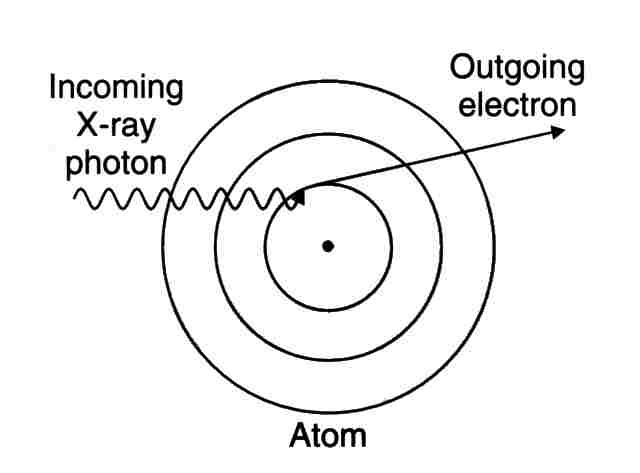
\includegraphics[width=7cm]{../Pictures/Chapter_2/photo_el_2}
\caption[Photo electric effect]{Phenomenology of the photo electric effect}
\label{fig:photo_electric}
\end{figure}
\newpage
\subsection{Compton scattering}

Compton scattering is the inelastic scattering of the incoming photon with a weakly bound electron in the material (see figure \ref{fig:compton}):
\begin{equation}
\gamma + atom \rightarrow (\gamma ') + e^{-} + atom^{*}
\end{equation}
Contrary to the photoelectric effect, this only concerns quasi-free electrons of the material. 
The photon transfers part of its energy to the electron, which is freed from its shell.
Applying conservation of energy and momentum it is possible to derive the energy of the scattered gamma as well as the direction and energy of the freed electron.
\begin{equation}
E_{\gamma '} = \frac{E_{\gamma}}{1+\frac{E_{\gamma}}{m_{e}c^{2}}(1-cos\theta)}
\end{equation}
The angular distribution can be described by the Klein-Nishina formula. It can be noted that forward scattering direction are favoured as the incoming photon energy increases
\begin{equation}
\frac{d\sigma _{cpt}}{d\omega} = Z \cdot \frac{e^{2}}{4\pi \epsilon _{0} m_{e} c^{2}} \cdot \frac{1}{2} \cdot \frac{E'_{\gamma}}{E_{\gamma}} \left( 1 - \frac{E'_{\gamma}}{E_{\gamma}} \cdot sin^{2}\theta + \left[ \frac{E'_{\gamma}}{E_{\gamma}} ^{2} \right] \right)
\end{equation}
The total cross section can be computed by integrating the differential cross section over the angle, with $\epsilon = h\nu / mc^{2}$ and $r_{e} = h/mc$.
\begin{equation}
\sigma _{KN} = 2\pi r_{e}^{2} \left{ \frac{1+\epsilon}{\epsilon ^{2}} \left[ \frac{2(1+\epsilon)}{1 + 2\epsilon} - \frac{ln(1+2\epsilon)}{\epsilon}\right] + \frac{ln(1+2\epsilon)}{2\epsilon}-\frac{1+3\epsilon}{(1+2\epsilon)^{2}}\right]
\end{equation}
\begin{figure}
\centering
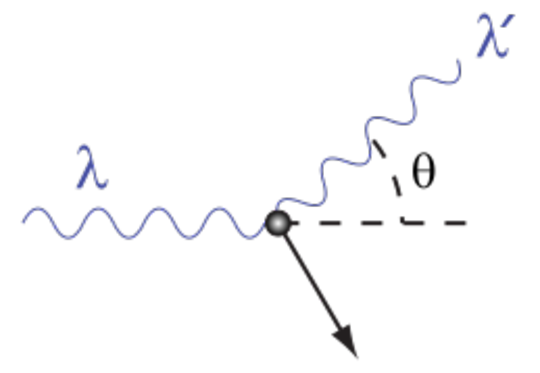
\includegraphics[width=7cm]{../Pictures/Chapter_2/259px-Compton-scattering.pdf}
\caption[Compton scattering]{Phenomenology of Compton scattering}
\label{fig:compton}
\end{figure}

\subsection{Pair production}

If the energy of the gamma exceeds $2m_{e}c^{2} = 1.02$ MeV, the impinging photons can also be converted into an electron-positron pair. The cross-section of the pair production is given at low energies (thus low screening) by
\begin{equation}
\sigma _{pair} = 4\alpha r_{e}^{2} Z^{2} \left( \frac{7}{9}ln2\frac{E}{m_{e}c^{2}} - \frac{109}{54}\right)
\end{equation}
The cross section is very low compared to that of photoelectric and Compton effect until the energy of the $\gamma$ approaches several electron Volts. Thus for the energies involved in medical applications pair production can be neglected.
The measuredcross section for the processes considered is shown in \ref{fig:cross_section} for Lead. 

\begin{figure}
\centering
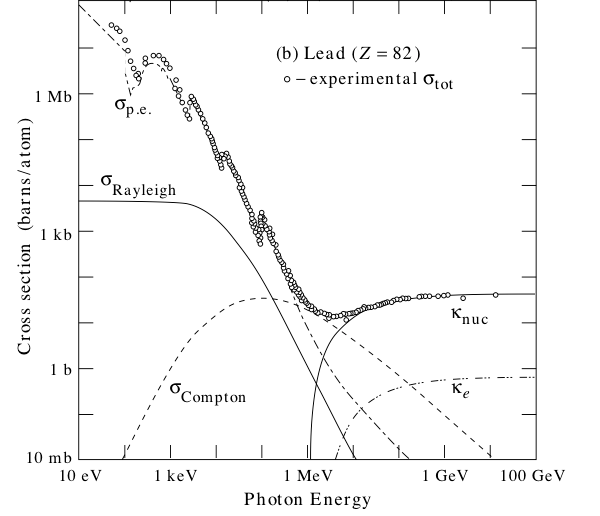
\includegraphics[width=9cm]{../Pictures/Chapter_2/sigma_gamma.pdf}
\caption[$\gamma$ cross section]{Cross section for the different processes in lead}
\label{fig:cross_section}
\end{figure}
\newpage
\section{The scintillation mechanism}

As a general idea the scintillation process can be considered as the conversion of the energy of an incident $\gamma$ quantum or particle into a certain number of low energy photons \cite{Rodnyi1997}. In a way it can be therefore defined as a wavelentgh shifting process \cite{Lecoq2006}.

\begin{figure}
\centering
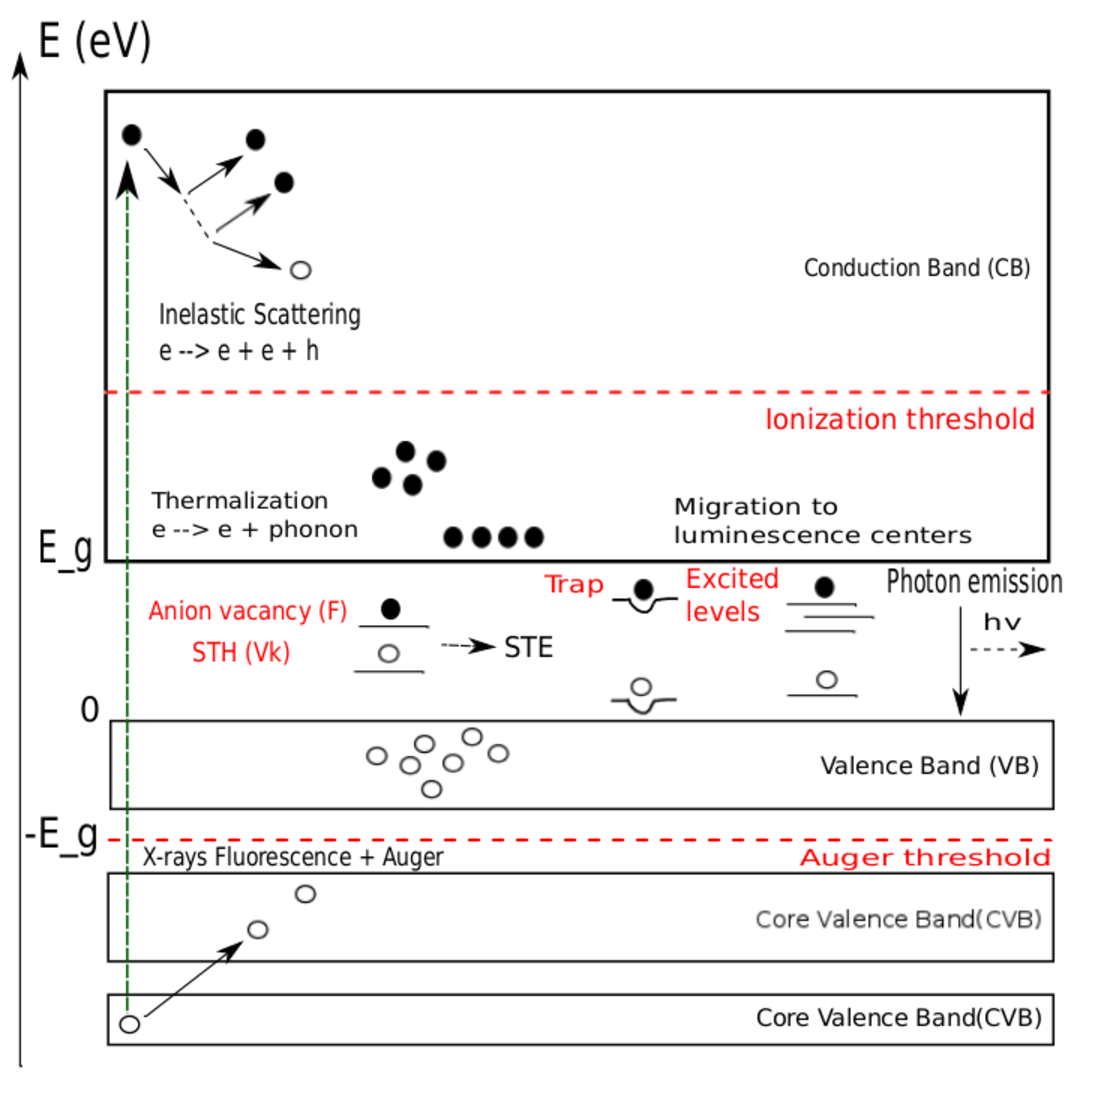
\includegraphics[width=12cm]{../Pictures/Chapter_2/drawing_2.pdf}
\caption[Energy deposition in scintillator]{Chain of energy deposition processes in crystals}
\label{fig:lecoq_easy}
\end{figure}

After a ionization event, generated by the mechanisms presented above in the case of a $\gamma$ interaction, the scintillator relaxes towards a new equilibrium. This process is characterized by a multitude of sub processes, that can be depicted by band diagrams as the one in figure \ref{fig:lecoq_easy}.
As long as the energy of the particles is high enough, it is transferred to secondary particles of lower energy, creating an electromagnetic cascade.
A crystal is an ordered ensemble of atoms, and the electrons in the KeV range start to couple with electrons and atoms of the lattice. As a result of their interaction with electronic states of the material, couples of electrons and relative vacancies are created. The electron hole pairs migrate in the lattice above and below the ionization threshold until they are trapped by a defect or recombine on a luminescent center. Alternatively they cool down by coupling to the lattice vibrations until they reach the top of the valence band (hole) or the bottom of the conduction band (electron). They can also form loosely bound structures called exciton, with en energy slightly smaller than the bandgap energy.
The scintillator itself must contain luminescent centers, either intrinsic or extrinsic (doping ions). These molecular systems in the lattice present characteristic radiative transitions between excited states.
Recombination brings the release of optical photons, at characteristic wavelengths.
%
%The scintillation process can therefore be represented as the sequence of the following stages\cite{Rodnyi1997}: 
%
%\begin{itemize}
%\item Absorption of ionizing radiation and creation of primary e-h pairs
%\item Relaxation of primary e-h pairs with production of secondary e-h pairs, plasmons, photons, etc.
%\item Thermalization of low energy e-h pairs down to the band gap energy $E_{g}$
%\item Energy transfer form the e-h pairs to the luminescence centers
%\item Emission of scintillation photons
%\end{itemize}

\subsection{Creation of electron hole pairs}

To analyze more in depth the mechanisms of the scintillation, we can consider an intermediate energy $\gamma$ ray ( $\sim 500$ KeV) interacting with the scintillator material. In this case the photoelectric effect is dominant. Thus it will produce a hole in a inner shell (usually K shell) and a free or quasifree electron.
\begin{equation}
A + h\nu \rightarrow A^{+} + e
\end{equation}
The energy of the primary electron will be $h\nu - E_{k}$ where $E_{k}$ is the K level energy. The relaxation then happens differently for electrons and holes. 

The ionized atom ($A^{+}$) can relax either radiatively, thus emitting a photon, or nonradiatively, generating a secondary electron. This is know as the Auger effect. Thereafter a cascade of both radiative and nonradiative processes takes place.
The Auger electron and the primary electron begin a proces of electron-electron scattering or phonon emission. In the case of a radiative emission, the soft x-ray photon emitted may be absorbed producing a new deep hole and free electron. 

The electron on the other hand will ionize an atom
\begin{equation}
A + e \rightarrow A^{+} + 2e
\end{equation}
The two undistiguishable electrons will undergo a number of other ionization processes, resulting in an avalanche of secondary electrons and holes. At some point the secondary products of these processes are not able to ionize the medium anymore.
A fast electron can in principle interact also with valence electrons of the medium, producing collective oscillations known as plasmons. Plasmons behave as quasiparticles, with an energy of $\sim 10$ eV and can decay into e-h pairs.

This ensemble of avalanche processes continues until the generated secondaries are not able to create further ionization. At this point electrons and holes start to interact with the vibrations of the lattice in a stage called thermalization, via different mechanisms of electron-phonon interaction. 
 As a consequence, at the end of this chain of de-excitation processes, low energy electronic excitations are present: electrons in the conduction band, holes in the valence band, valence excitons, core excitons.
 
\subsection{Intrinsic luminescence}

\begin{figure}
\centering
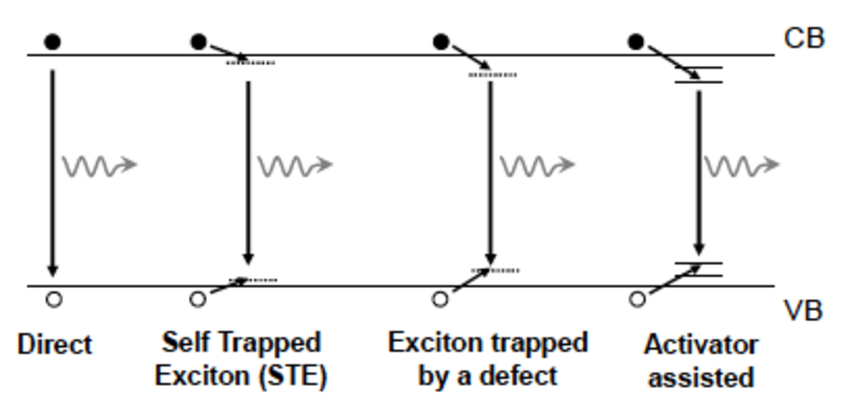
\includegraphics[width=12cm]{../Pictures/Chapter_2/traps.pdf}
\caption[Electron hole recombination]{Different processes for electron hole recombination}
\label{fig:traps}
\end{figure}
Electron and holes have several ways to recombine after thermalization and give rise to scintillation photons.
The simplest emission process is direct recombination
\begin{equation}
e + h \rightarrow h\nu
\end{equation}
Recombination can more effectively take place when the energy of the electron and hole has decreased, so that they form an exciton. 
However the various impurities and lattice defects play a very important role in the scintillation process. Thermalized carriers can be bound in some places of the lattice where atom or defects are localized. 
For example many ionic crystals shows phenomena of localization of the valence hole in the lattice, known as self-trapping. This structure appears when a thermalized hole localizes an anion, polarizing the environment. As a result the hole can be shared between two neighbouring ions forming a $V_{k}$ center, and the hole is defined as self-trapped hole. For high energy excitation direct creation of valence exciton is unlikely, so $V_{k}$ centers usually capture free electrons. From subsequent de excitation they can emit photons, thus giving rise to the excitonic luminescence.
\begin{equation} 
e + h \rightarrow ex \rightarrow h\nu
\end{equation}

\subsection{Core to valence transitions}

If the core bands of the scintillator lie below the Ager threshold, the most favoured transitions involve holes in the valence band and electron in the conduction band. Nevertheless some systems present the so-called cross luminescence. This phenomenon implies a direct core to valence transition, due to the fact that holes in uppermost core bands can not de excite non radiatively \cite{Lecoq2006}. 

A notable example of core to valence transition is $BaF_{2}$. In this system a $Ba^{2+}$ $5p$ core hole is above the Auger threshold and hence Auger effect does not occur. They can recombine directly with electrons from the valence band, in most of the cases radiatively.
This leads to a very fast luminescence given by recombination of the core hole, while the primary electron de excitation is more complex thus leading to a slower component.

\begin{figure}
\centering
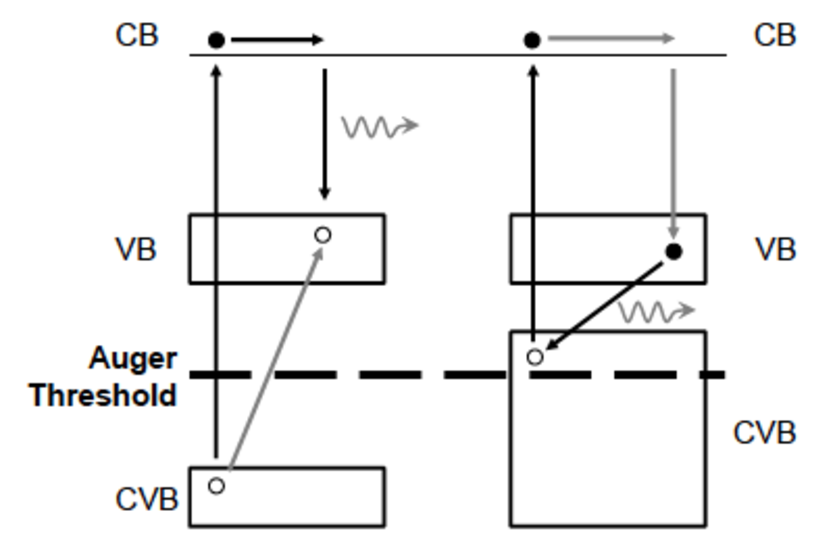
\includegraphics[width=8cm]{../Pictures/Chapter_2/core_to_valence.pdf}
\caption[Core to valence luminescence]{Direct luminescence (left) versus cross to valence luminescence (right)}
\label{fig:CTV}
\end{figure}
 

\subsection{Extrinsic luminescence}

Most of the scintillator samples used in this work are extrinsic, that is doped with activation centers that can enhance the intrinsic scintillation properties presented above by favouring direct recombination.
Rare earth ions doping, for example, is largely used in scintillator technology because of the parity and spin-allowed transition $4f^{n-1}5d\rightarrow 4f^{n}$. 
Extrinsic scintillators usually present different luminscent mechanisms driven by activated sites \cite{Lecoq2006}:
\begin{itemize}
\item $e + h + A \rightarrow ex + A \rightarrow A^{*} \rightarrow A + h\nu$
\item $e + h + A \rightarrow A^{1+} + e \rightarrow A^{*} \rightarrow A + h\nu$
\item $e + h + A \rightarrow (A^{1-})^{*} + h \rightarrow A + h\nu$
\item $A \rightarrow A^{*} \rightarrow A + h\nu$
\end{itemize}
In the first case the insertion of dopants is able to sufficiently quench the exciton luminescence so that excitation of radiative centers results form a transfer from excited matrix states.
A competing process is the direct capture of free thermalized carriers by luminescent center, in the case of electrons or holes.
In heavy doped or self-activated crystals ($CeF_{3}$) direct excitation by ionizing radiation is possible.

%QUI MANCA QUALCOSA!

\subsection{Quenching phenomena}
TO DO
% thermal, concentration, trapping Chapter3 Lecoq
\section{Operational parameters}
\subsection{Light yield}
One of the feature commonly required of a scintillator is to have a high light yield, that is to be an efficient converter of radiation to visible light.
In this case the relative light output of the scintillator, $L_{R}$, can be considered the significant quantity. It is defined as the number of emitted photons per unit of absorbed energy \cite{Rodnyi1997}
\begin{equation}
L_{R} = \frac{N_{ph}}{E_{\gamma}}
\end{equation}
The number of produced e-h pairs $N_{eh}$ depends on the average energy needed for the creation of a low energy e-h pair, $\chi _{eh}$. This value depends on the type of lattice and band gap of the material, with a numerical coefficient $\beta$
\begin{equation}
\chi _{eh} = \beta \cdot  E_{g}
\end{equation}
If $\alpha$ is the average number of scintillation photons produced by a single e-h pair, the light output is
\begin{equation}
L_{r} = \frac{\alpha \cdot N_{eh}}{E_{\gamma}} = \frac{\alpha}{\chi _{eh}} = \frac{\alpha}{\beta \cdot E_{g}}
\end{equation}
The coefficient $\alpha$ depends on the transport efficiency of the e-h pairs to the luminescence center and the conversion efficiency of the center itself.

\subsection{Optical properties and light transport}
% MANCA QUALCOSA!
TO DO
\subsection{Energy resolution and nonproportionality}
In the case of $\gamma$ spectroscopy it is necessary to discriminate quanta with different energy.
For scintillation detector this fundamental property is characterized by the energy resolution $R$, defined as $\Delta E/E$ (in $\%$) where $\Delta E$ is the full width at half maximum (FWHM) at pulse height $E$.
It depends on the characteristics of the scintillator, i.e. materials, size and defects as well as the coupling with the photo detector and the parameters of the photo detectors itself. Statistical fluctuations at any step of the detector chain, from dynode multiplication to photo cathode efficiency in the case of a PMT can worsen the resolution at the peak. 
Thus energy resolution can be defined as \cite{Rodnyi1997}
\begin{equation}
R^{2} = R_{S}^{2} + R_{PM}^{2} = R_{S}^{2} + \frac{\delta}{E_{\gamma}}
\end{equation}
where $R_{S}$ and $R_{PM}$ are, respectively, the scintillator and photomultiplier contributions and $\delta$ includes photo electron statistics.
It is possible to further decompose the scintillator resolution $R_{S}$ to take into account the factors depending on the type of scintillator used. In particular it is useful to introduce a term for the transfer efficiency of the optical photons $R_{S}$, a term for inhomogeneity $R_{i}$ and a term for nonproportionality $R_{n}$
\begin{equation}
R_{S}^{2} = R_{t}^{2} + R_{i}^{2} + R_{n}^{2}
\end{equation}
The interest lies in the fact that the two terms, for inhomogeneity and nonproportionality, account for the intrinsic resolution of the crystal.
Inhomogeneity arise from possible imperfections of the scintillator, such as local variations in the concentration of the dopant or optical defects.

Non proportionality arise when scintillators show deviation from stability of excitation spectrum, that is when linearity between energy of the excitation and relative light output is not preserved. This is particularly important for low energy excitation, since scintillation phenomena occur mainly on the surface. Non proportionality is caused by the statistical nature of the creation of secondary electrons and photons and contribute to worsen the resolution.

\subsection{Cerenkov effect}
Cerenkov radiation brings important information both in high energy physics and time resolved PET.
Cerenkov radiation occurs when a charged particle passes through a dieletric medium at a speed greater than the phase velocity of light in that medium.
The phase velocity of light in a medium of refractive index $n > 1$ is
\begin{equation}
v_{p} = \frac{c}{n}
\end{equation}
A charged particle can travel faster than the speed of light if, given its velocity $v_{p}$ 
\begin{equation}
\frac{c}{n} < v_{p} < c
\end{equation}
This translates to the following condition for the $\beta$ coefficient of the particle
\begin{equation}
\beta = \frac{v_{p}}{c} > \frac{1}{n}
\end{equation}
For a particle of a given mass thus the energy threshold is
\begin{equation}
K_{thr} = mc^{2}\left( \frac{\sqrt {n^{2}-1}}{n} - 1 \right)
\label{eq:thr}
\end{equation}
The phenomenology of Cerenkov effect can be explained considering the polarization of the medium caused by a charged particle traversing it.
Below the Cerenkov threshold the dipoles surrounding are symmetrically arranged around the path. As the particle crosses the threshold it travels faster than the speed at which it interacts with the dipoles. This symmetry breaking leads to a non-vanishing dipole moment and thus to the formation of a wave front.

\begin{figure}
\centering
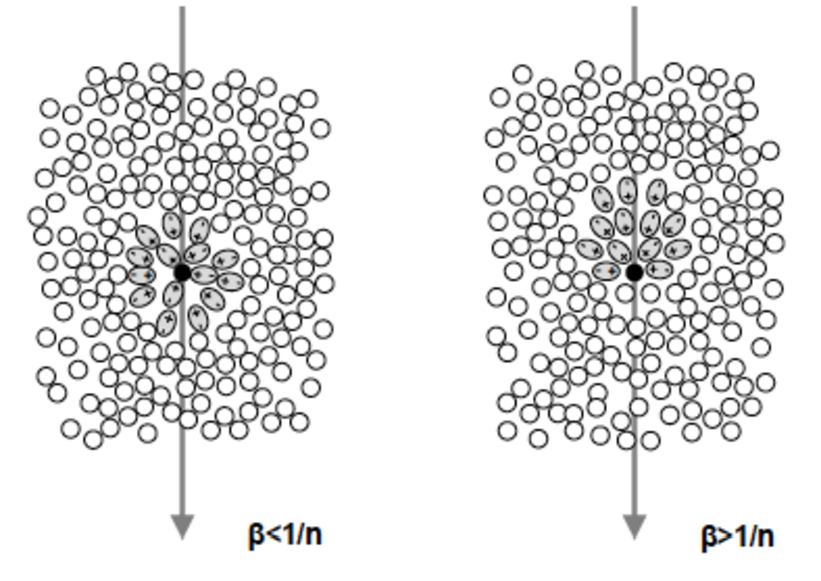
\includegraphics[width=9cm]{../Pictures/Chapter_2/cerenkov.pdf}
\caption[Cerenkov effect]{Phenomenology of Cerenkov effect}
\label{fig:cerenkov}
\end{figure}

Cerenkov photons are emitted at a characteristic angle in the forward direction, obtained via simple geometrical considerations. The distance traveled by the charged particle in a time $t$ is $t\cdot \beta \cdot c$ whereas the distance along which the photon propagates is $t\cdot c /n$ as shown in figure \ref{fig:cone}.
Therefore the characteristic angle at which photons are emitted can be calculated as
\begin{equation}
cos(\theta _{C}) = \frac{t c/n}{t \beta c} = \frac{1}{n\beta}
\end{equation}
As will be shown in the next chapter, the direction of emission retains a primary interest in the field of particle identification, while it has a negligible impact on timing measurement in PET scanners. It is worth to be noted that the Cerenkov photons are emitted promptly, taking a relevant share of the first incoming photons.  
\begin{figure}
\centering
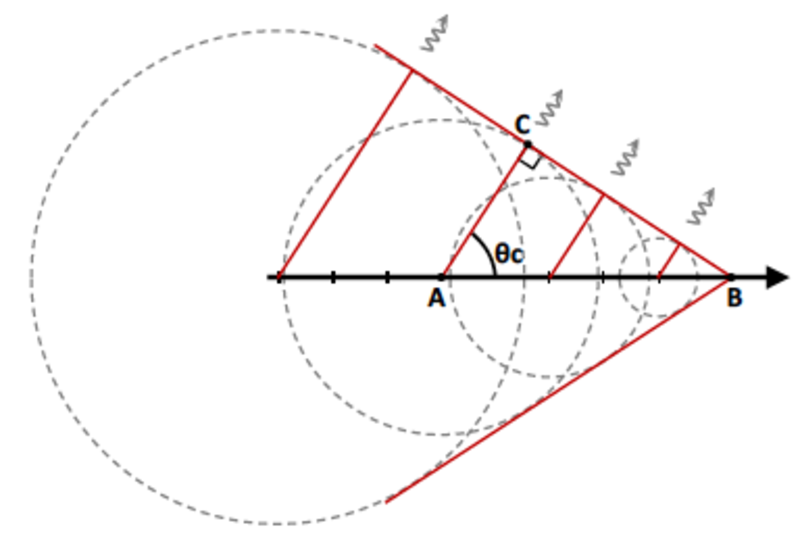
\includegraphics[width=9cm]{../Pictures/Chapter_2/cone.pdf}
\caption[Cerenkov emission cone]{Sketch of the Cerenkvo emission cone}
\label{fig:cone}
\end{figure}
It is useful to consider the number of emitted photons per unit length by a charged particle as a function of the wavelength
\begin{equation}
\frac{dN}{d\lambda dx} = \frac{2\pi z^{2}\alpha}{\lambda ^{2}}\left( 1 - \frac{1}{\beta ^{2}n^{2}(\lambda)} \right)
\end{equation}
Neglecting dispersion in the medium, and integrating over an appropriate interval of wavelengths we obtain that the photons are emitted mostly in the UV range.
\begin{equation}
\frac{dN}{dx} = 2\pi z^{2} \alpha \left( 1-\frac{1}{\beta ^{2} n^{2} (\lambda)}\right) \int _{\lambda _{1}} ^{\lambda _{2}} \frac{d\lambda}{\lambda ^{2}}  = 2\pi z^{2}\alpha sin^{2}\theta _{C} \left( \frac{1}{\lambda _{1}}-\frac{1}{\lambda _{2}}\right)
\label{eq:number}
\end{equation}

A simple calculation shows that, even at the low energies that characterize a PET exam (511 KeV), a non negligible number of Cerenkov photons is produced.
As an example, it is interesting to consider the case of the most popoluar crystal for PET detectors, Lu$_{2}$SiO$_{5}$:Ce (LSO) with a density $\rho _{LSO}$ = 7.48 g/cm$^{3}$ and a refractive index of 1.82 \cite{jellison2012}.
Given the K-shell binding energy of the electron (63 KeV \cite{xdata2009}), we can estimate, with the help of formula  \ref{eq:thr}, the energy threshold for Cerenkov production for electrons at 448 KeV.
If we then consider a freed electron from the K-shell and its average range in LSO (265 $\mu$m \cite{nist2005}), we can make use of formula \ref{eq:number}, given that
\begin{equation}
sin ^{2}(\theta _{c}) = 1 - \frac{1}{n^{2}\beta ^{2}} = 0.58
\end{equation}
The number of optical photons produced in the wavelength range 180 - 800 nm is $\sim$ 40.


\section{Most common scintillation processes}
The main crystal species used in this study will be briefly presented in this section, in particular with respect to the scintillation mechanism. Light yield and time profiles will be more deeply analyzed in the next chapters.
% magari puoi anticipare due cose sulle terre rare?
\begin{itemize}
\item \textbf{Lutetium Oxiorthosilicate}: Lutetium oxyorthosilicate (LSO) is a widely used crystal for PET detection and high energy phisics. The crystal structure of Lu$_{2}$Si0$_{5}$:Ce the Lu atoms occupy two equally-populated, crystallographically independent sites, and the Cerium doping atom is assumed to substitute for the Lutetium atom \cite{Naud1996}.
The 5d level is split by the crystal field of the host lattice into 3 sublevels, and the 4f ground state is split by the spin-orbit interaction into two levels.
The luminescence of LSO is due to parity-allowed electric dipole transitions from the lowest 5d sublevel to the split 4f ground state, with emission band at 410 nm.
Due to the high density (7.4 g/cm$^{3}$), very fast emission ($\sym$ 40 ns) and high light yield ($>$40000 photons/MeV) is considered to be on the most important crystals for calorimetry.
\item \textbf{Lutetium Aluminum Garnet}: Lutetium Aluminum Garnet (Al$_{5}$Lu$_{3}$O$_{12}$) has been recently proposed as a candidate for future calorimetry experiment\cite{Kris2013}, for the high density (6.73 g/cm$^{3}$) and fast emission profile of the main components ($<$ 60 ps).
LuAG crystals present relevant intrinsic and extrinsic scintillator characteristics.
The intrinsic scintillation of LuAG comes from processes related to self trapped exciton de excitation. Indeed in case of strong electron hole coupling to the lattice a carrier can be trapped in its own field.
STEs in LuAG lead to absorption band at 7.1 and 7.3 eV and emission upon recombination at 5 eV.
STEs may also localise around Lu$_{Al}^{3+}$ defects and give rise to emission at 3.3 eV.
This recombination mechanisms are very slow, usually $\sym$ 2 $\mu$s and for this reason the LuAG lattice is often doped, as the case of LSO with a rare earth activator (Yb, Pr, Ce).
In particular we will consider the case of Cerium and Praseodymium doping.
The case of Cerium doping is similar to the LSO case, with an emission band peaking at 520
nm that corresponds to the Ce$^{3+}$ 5d$\rightarrow$4f transitions.
In the case pf Praseodymium doping, apart from the excitonic luminescence, two bands are present, corresponding to the Pr$^{3+}$ 4f5d$\rightarrow$4f$^{2}$ and 4f$^{2}\rightarrow$4f$^{2}$ contained respectively in the 285-450 nm band and 450-880 nm band \cite{Drozdowski2008}. For calorimetry application only the first is relevant. 
\item \textbf{Cerium Fluoride}:
\item \textbf{Bismuth Germanate}: Bismuth Germanate (Bi$_{4}$Ge$_{3}$0$_{12}$), or BGO, is been considered for many years the gold standard for radiation detection, in nuclear medicine and high energy physics, because of its high density (7.13 g/cm$\^{3}$), high scntillation output ($>$20000 photons/MeV) and relatively fast emission (two components, main one $\sym$300 ns).
BGO is an intrinsic scintillator, that is no dopant is added. The observed fluorescence is assigned to $^{3}$P$_{1}\rightarrow ^{1}$S$_{0}$ transitions of Bi3$^{+}$, with broad emission band at 490 nm \cite{Weber1996}.
\end{itemize}